\documentclass{beamer}
\usetheme{metropolis}

\usepackage{calc}
\usepackage{enumitem}
\usepackage{graphicx}
\usepackage{textcomp}
\usepackage{hyperref}
\hypersetup{colorlinks = true, linkcolor = .}

\title{Alshayun: A mobile education application}
\date{March 20, 2019}
\author{Jacob Chappell}
\institute{University of Kentucky}

\begin{document}

\maketitle

\section{Introduction}

\begin{frame}{What is Alshayun?}
    \begin{itemize}
        \item A mobile application for delivering articles consisting of rich
            text and interactive \textbf{applet}s to \textbf{reader}s.
        \item Designed for three actors in mind (a user is any of them):
            \begin{description}[leftmargin=!,labelwidth=\widthof{\bfseries Content Author}]
                \item[Content Author] Anyone who has anything about which they
                    would like to write.
                \item[Reader] Anyone who would like to read what one or more
                    \textbf{content author}s have to say.
                \item[Developer] Anyone capable of developing \textbf{applet}s
                    and other functionality of \textbf{Alshayun} of which
                    \textbf{content author}s and \textbf{reader}s can make use.
            \end{description}
    \end{itemize}
\end{frame}

\begin{frame}{Inspiration}
    \begin{itemize}
        \item My fascination with Bézier curves led me to the Internet.
        \item I discovered the article
            \href{https://pomax.github.io/bezierinfo/}{A Primer on Bézier
            Curves} by Pomax.
        \item I was intrigued by the interactive \textbf{applet}s weaved
            seamlessly throughout the text.
    \end{itemize}
    \begin{figure}
        \begin{center}
            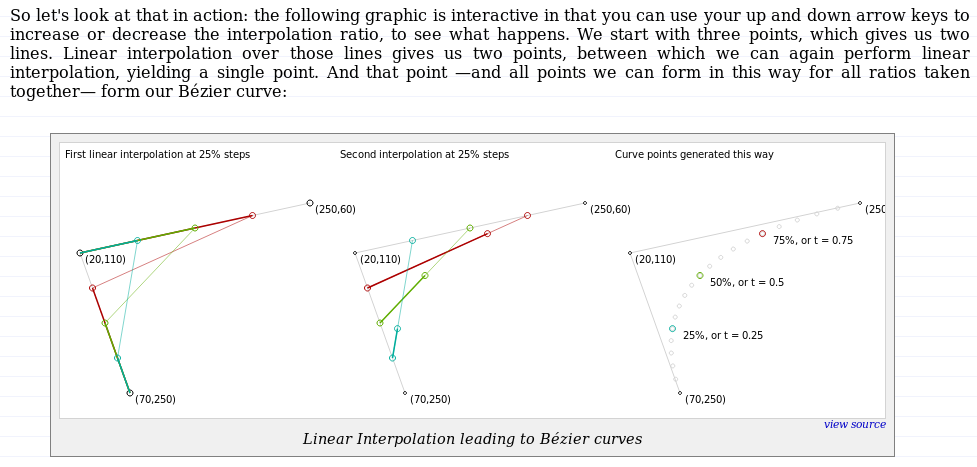
\includegraphics[scale=0.25]{images/pomax.png}
        \end{center}
        \caption{Example \textbf{applet}s from \textit{A Primer on Bézier
        Curves}.}
    \end{figure}
\end{frame}

\begin{frame}{About the Name}
    \begin{itemize}
        \item At inception, \textbf{Alshayun} was planned to be a mathematics
            education platform.
        \item I built a more general platform, but kept the original ``mathy'' name.
        \item
            \begin{center}
                \textbf{Origins of Algebra} \\
                Arabic (``al-jabr'')\textrightarrow Spanish\textrightarrow
                Latin\textrightarrow English
            \end{center}
        \item Arabic ``al-shayun'' appeared frequently in the original algebraic
            documents and means ``the unknown thing''; it became the ``x'' in
            Latin/English-speaking algebra (see
            \href{https://cosmosmagazine.com/mathematics/why-x-marks-unknown-0}{Why
            X marks the unknown} by Terry Moore).
    \end{itemize}
\end{frame}

\end{document}
